%===================================== CHAP 3 =================================

\chapter{Real time kinematic GPS}
This chapter will explain \acrfull{rtk-gps}, as well as how it's used in the automatic landing system. The first section will include a overview of the system, including the state of the current system. The next part will contain different reference frame used in the \gls{rtk-gps} module. Then the different \acrfull{gnss} system will be presented as well as atributes in the \acrfull{gps}. Then a quick overview over the different error sources that can affect a \gls{gnss} system, before the consept \acrfull{dgps} is presented. Lastly the term \gls{rtk-gps} will be explained.

In the following the behaviour of a receiver is denoted using terms rover and base station. The term base station means a receiver assumed to have a known position by the other receivers. The term rover means a receiver that is allowed to move, is the main focus for position estimation.
\section{System layout}
An integrated system required for automatic landing will typically consist of four main sub-systems as shown in figure \ref{figure:SystemOverview}. Today these systems are individually available or in development; however not integrated into a proven working system allowing for automatic landing of \glspl{uav}. The four main systems comprises of the navigation part, guidance part, control part and the user interface, where further validation and development of the first is the main topic for this work.

\begin{figure}[H]
	\centering
		
\includegraphics[width=0.7\textwidth]{figs/SystemOverview.png}
		\caption{The structure of the autonomos landing system}
		\label{figure:SystemOverview}
\end{figure}

The navigation system will apply \gls{rtk-gps} to estimate the relative position of the \gls{uav}. More details about what \gls{rtk-gps} is, will be given in \ref{ss:rtk-gps}.

The control and guidance system has currently only been tested in \gls{sil} simulations with Ardupilot, which shows promising result likely to be sufficient for automatic landing applications. However this module has not yet been implemented to support the use of \gls{rtk-gps} as required for performing automatic landing.

This work will identify and describe the navigation system necessary to allow for automatic landing of \glspl{uav}. The \gls{rtk-gps} solution will be compute by two different system ,which will be compared against each other. The first system is called Piksi, and is developed by Swift navigation. The second system will is called Rtklib, and is developed by T. Takasu. The latter is indepente on the type of receiver, and thus will be the main focus of this work. More detail about Piksi and Rtklib will be given in \ref{ss:Piksi} and \ref{ss:Rtklib}.

The comparison test will be used to summarize further work required for complete identification of gaps and work required for closure of these gaps such that a control system including provision for automatic landing may be developed and implemented in a integrated \gls{uav} control system. The \gls{uav} that will be used in the test is a Skywalker X8 Fixed Wing \gls{uav}. More details about the X8 will be given in \ref{ss:SkywalkerX8}


This work will identify and describe the gaps which will need to be closed on order to develop and implement a solution which will allow for automatic landing of \glspl{uav}. Two different system that will be compared against each other. 
The current state of the system is that it consist of two parts that has not yet been integrated with each other. The part were which is the main focus of this thesis is the positioning part. The plan is to use \gls{rtk-gps} for positioning estimation. The second part is the path and control path. Currently there has only been done simulation of the guidance system. It shows promising results, but is yet to be integrated with \gls{rtk-gps}. For more information on the subject please read the MSc thesis by \citep{Froelich}. Figure \ref{figure:SystemOverview} gives a overview on how the system may look like. Ideas on how the intergration can be acheived will be given in the future work section.
\section{Reference frames}
A \gls{gnss} system calculate a position estimated of where on the Earth the receiver is. For the position to have any meaning a reference system has to be defined where a frame can be consider as an inertial frame. From there a reference frame can be fixed to the Earth rotation, but for local navigation if must be referred to surface of the Earth. This section will present the different reference frame used in global navigation systems.
\subsection{ECI}
\gls{eci} frame is considered a inertial frame for terrestrial navigation. The origin is fixed in the center of the Earth, and the axis is fixed in space. This frame can be considered as a non-accelerating where Newton's laws of motion applies. 
\subsection{ECEF}
The \gls{ecef} coordinate system is defined in the center of the Earth with it's x-axis point toward the intersection between the Greenwich meridian and Equator ( $0\deg $ longitude, $0\deg $ latitude). The z-axis points along the Earth's rotational axis, and the y-axis complete the right handed orthogonal coordinate system. The \gls{ecef} system can be represented in either Cartesian coordinates (xyz) or ellipsoidal coordinates (longitude, latitude and height). The \gls{ecef} frame rotate relative to the \gls{eci} frame at a angular rate of $\omega_e = 7.2921 \times 10^{-5}rad/s$, where $\omega_e$ is the Earth rotation. Due to the relatively low rotation speed some system can consider the \gls{ecef} frame as inertial.
\begin{figure}[H]
	\centering
		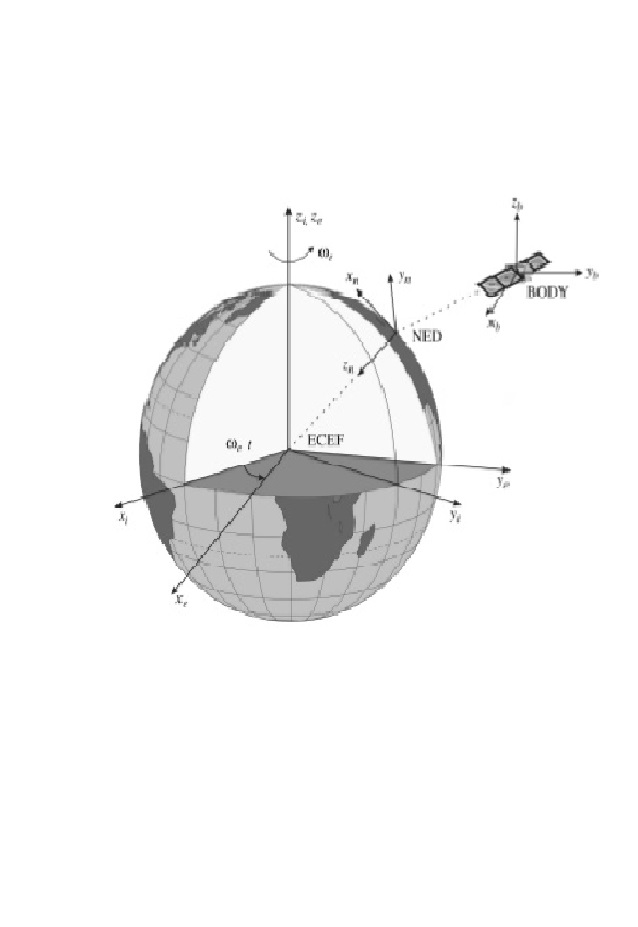
\includegraphics[width=0.7\textwidth]{figs/ECEF-Frame.jpg}
		\caption{The \gls{ecef} frame. Picture from \citep{fossen2011handbook}}
		\label{figure:ECEF}
\end{figure}
\subsection{Local reference frame}
The \gls{ned} and \gls{enu} frame is defined as relative to the Earth reference ellipsoid (\gls{wgs-84}). For the \gls{ned} frame the x axis points in the direction to the true North, y axis towards East while the z axis points downward to completed the right handed orthogonal coordinate system. The \gls{enu} has the x and y axis exchange place in respect of the \gls{ned} frame, and the z axis point upwards instead of downwards.
\section{GPS}
A quick overview of the gps and other gnss systems.
\subsection{GNSS constellations}
There are currently two operation \gls{gnss} constellations with global coverage, which is American \gls{gps} and Russian \gls{glonass}. Other \gls{gnss} constellations that will be operational in the near future is the Chinese BeiDou and European Galileo.
\subsection{GPS attributes}
The \gls{gps} satellites transmits continuously using two radio frequencies in the L-band referred to as \gls{l1} and {l2}. The L-band covers frequencies between 1 GHz and 2GHz, and is a subset of the \gls{uhf} band.

Previously only the \gls{l1} signal was intended from civil users, but in the future a new {l2} signal as well as the \gls{l5} signal will be available for civil users. 

\gls{gps} uses it's time reference called \gls{gpst}, which is independent from the \gls{utc}. Because of this independent the \gls{utc} diverge away from the \gls{gpst}, and to correct this the \gls{gps} keeps track of the offset between \gls{gpst} and \gls{utc}. The offset is included in the \gls{gps} message as leap seconds to be added to the \gls{gpst}. \gls{gpst} can be given as \gls{tow}, which include the number of weeks since 1980-01-06T00:00Z. \gls{tow} is given in seconds, and is reset each week when the week number is incremented. More information about the \gls{gps} can be found in \citep{GPSBOOK,vik2014integrated} 

The two basic ways to measure the psedurange is code and phase measurement. Phase measurement is the most accurate of the two, but also least reliable.
In code measurement the information in signal is used to calculate the psudorange between the receiver and the satellite. In phase measurement the signal itself is used to calculate the psudorange by counting the number of cycles between the receiver and the satellite. It's phase measurement that is used in \gls{rtk-gps}.

The receiver needs at least four satellite to be able to estimate the receiver position. Three of the satellite is used for the position, and the fourth if used to calculate the receiver clock bias. 
 
\section{Error sources}
In order to get high accuracy in the position estimation the different error sources must be identified and removed if possible. This section will identify some of the larger error sources that can affect the \gls{gps} signal, and how to remove or mitigate them in the estimation.
\subsection{Clock error}
There is drift in both the satellite clock and the receiver clock. The atomic in the satellites makes the clock drift negligible from the user perspective. The receiver clock tend to drift, and if not taken into account will cause large deviations in the position estimate from the true position. This error is remove by including a fourth satellite in the position computation. The satellite clock error given in the satellite message. 

\subsection{Ionospheric and Trophospheric Delays}
When the \gls{gps} signals travel though the atmosphere there will be a delay caused by the different layers, as further explained in this section.
\subsubsection{Ionospheric delay}
Gas molecules in the ionosphere becomes ionized by the ultraviolet rays that is emitted by the sun, which release free electrons. These electron can influence electromagnetic wave propagation, such as GNSS signals. The delay that the single get from the ionosphere may cause a error the the order of $1-10 meters$. The error can be mitigated by using a double frequency receiver, or by applying a mathematical model to estimate the delay. Both those cases is with a single receiver, but by having a second receiver the GNSS solution system can assume that both receiver receive signal in the same epoch, which means that the signals have experienced the same delay. More on this in section \ref{ss: Error mitigation DGPS}.

\subsubsection{Tropospheric delay}
The tropospheric delay is a function of the local temperature, pressure and relative humidity. The delay can vary from $2.4$meters to $25$ meters depending on the elevation angle of the satellites. The error can be mitigated by applying a mathematical model to estimate the tropospheric delay, and by using a elevation mask can remove all satellites with a elevation angle bellow a certain threshold. Error caused by tropospheric delay can be removed in the same manners as ionospheric delay when using two or more receivers. More on this in section \ref{ss: Error mitigation DGPS}.

\subsection{Ephemeris Errors}
A satellite isn't able to perfectly follow a given orbit, and therefore there will be a deviation between satellite position given to the receiver and the true position of the satellite. This is called the ephemeris error. The true position of a satellite is monitored and corrected by the owner of the \gls{gnss} constellation, but error between each correction can be expected.
\subsection{Multipath}
One of the primary source of error in in a GNSS receiver is multipath. Multipath happens when the satellite signal is reflected by a nearby surface before if reach the antenna. The delay introduced in the signal can make the receiver believe that its position is several meters away form its true position. The easiest way to mitigated multipath is to place the antenna at a location with open skies, and not tall structures nearby.
\section{Dilution of Precision}
The geometry of the \gls{gnss} constellation affect the accuracy of the position solution. Pore geometry will also enhance the effect that different error sources has on the position solution.
\section{Differential GPS}
Differential GPS consist of at least two receivers, where one is called a base station and the rest rovers. The two receivers are within range of a communication channel over which they are communicating. Figure \ref{figure:DGPS} gives an example on \gls{dgps}. The base station has a known position, and the rover estimate the baseline from itself to the base station. 
\begin{figure}[H]
	\centering
		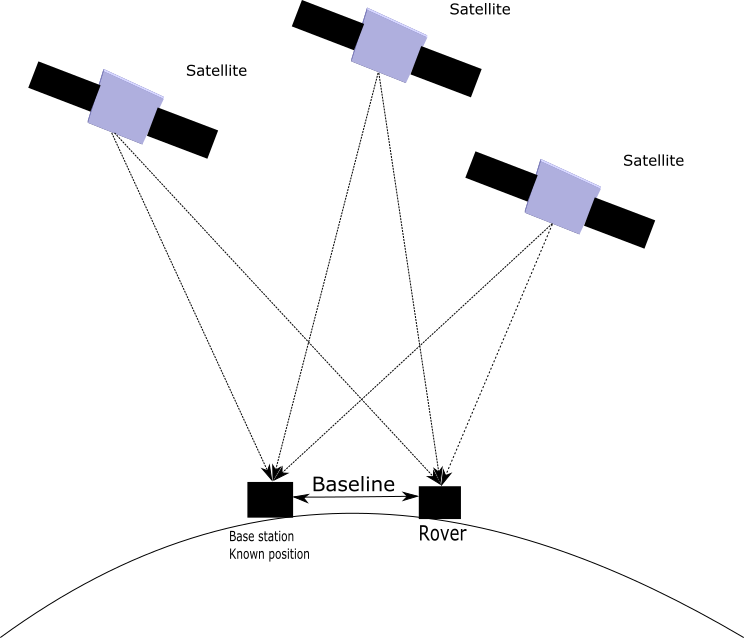
\includegraphics[width=0.7\textwidth]{figs/DGPS.png}
		\caption{Concept figure of DGPS}
		\label{figure:DGPS}
\end{figure}
\subsection{Integer Ambiguity Resolution Strategy}

Write first why the resolution of the integer ambiguity is important:

The integer ambiguity is the uncertainty of phase cycles between the receiver and the satellites.

There are several strategies on how to resolve the integer ambiguity. A well used strategy is the \gls{lambda} method. \gls{lambda} starts by reducing the integer search space by decorrelation adjustment. The \gls{lambda} method has two types of outputs. One is called the fixed solution, and the other is called the float solution. The float solution is the first solution given by the \gls{lambda} method and is used to find the fixed solution. When the right fixed solution is reached the position estimation in from a \gls{dgps} can be considered highly accurate. The solution program can calculate the wrong fixed solution, or experience a cycle slip (\ref{figure:CycleSlip}). In order to reduce the possibility of letting a wrong solution become the fixed solution the program need a good integer ambiguity validation strategy. One validation strategy is to check if the ratio between the best ambiguity estimate and the second best estimate in greater then a certain threshold. High \gls{dop} will effect the time the LAMBDA method needs to find a fixed solution.

\subsection{Cycle slip}\label{ss:cycleSlip}
When the integer number of cycles experience a sudden jump in value due to loss of lock of a receiver phase lock it's called cycle slip. The effect of cycle slip is a bias in the measurement large enough to make navigation difficult. The effect of cycle slip will appear as seen in figure \ref{figure:CycleSlip}.
\begin{figure}[H]
	\centering
		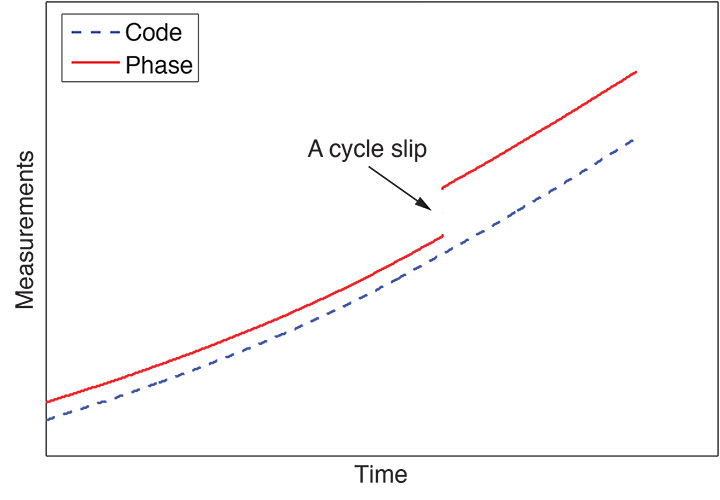
\includegraphics[width=0.7\textwidth]{figs/cycleSlip.jpg}
		\caption{The \gls{ecef} frame. Picture from \url{http://gpsworld.com/wp-content/uploads/2014/01/I-Fig1.jpg}}
		\label{figure:CycleSlip}
\end{figure}
\subsection{Error mitigation in DGPS} \label{ss: Error mitigation DGPS}
The advantage with DGPS is that two or more receivers can share the same error sources. This enable the solution system almost completely remove them.
In the case of a moving baseline situation the GNSS system assumes that the rover is close enough to the base station such that they shear the same atmospheric conditions. If this assumption holds the system should be able to almost remove the error caused by atmospheric delay.


\subsection{RTK GPS}\label{ss:rtk-gps}
\gls{rtk-gps} provide accurate baseline position estimation in real time. Can either have a kinematic setting or a moving baseline setting. The difference between the two is that in kinematic the base station has a known stationary position, while in moving baseline the base station position is unknown and allowed to move. The advantage with the moving baseline configuration is that \gls{rtk-gps} can be used to find the relative position between two dynamical system using \gls{gnss} in real time. This will be the case in automatic ship landing system, where the base station must be allowed to move. Also to determine the exact position of a base station require a long measurement period. The advantage with kinematic mode is that it can give a more accurate position estimate.

\gls{rtk-gps} systems needs to calculate the position estimate quicker then a standard  system. This is done by sacrificing the correctness of the solution, however in the resent time efficient software and hardware has reduced the this factor.

In a \gls{rtk-gps} set-up the rover assumes that it's receive the \gls{gnss} signals at the same time as the base station, and thus the two receivers receive the same signal without it having been altered any more disturbance, except local disturbance like multipath. This puts a restriction on the the range of the baseline. The assumstion that the two receiver share the same disturbance is valid for a baseline up to $2km$
\cleardoublepage